\section{Proposed Method}

In this section we will give to the lecturer a detailed description of the proposed algorithm: 
some implemented procedures will be explained through pseudocode. 
The algorithm works in successive stages as described in the following:

\begin{itemize}
    \item Kernel loading
    \item Image reading
    \item Output Image creation
    \item Image selection, enlargement and filling
    \item Image enhancement
\end{itemize}

The algorithm is implemented in C++ and CUDA, it is divided into two parts: the first one focuses on the CPU, which is responsible for the reading of the image
and the kernel loading; the second one is the GPU part, which is responsible for the image cut out, enlargement, filling, and enhancement.
The inputs required by the application are based on the commands given by the user through the command line, and they are the following:
\begin{itemize}
    \item The path of the image to be zoomed;
    \item The -$c$ (--$custom$) flag, which chooses a custom kernel, followed by the file path of the kernel;
    \item The -$g$ (--$gauss$) flag, which chooses a Gaussian kernel, followed by the length of the kernel and the $\Sigma$ value, mutually exclusive with the previous;
    \item An optional $v$ character, appended to the mode, which enables the verbose mode;
    \item An optional $f$ character, which forces the use of global memory instead of the shared;
    \item The coordinates of the center of the cut-out area, in the form of $x,y$;
    \item The width and the height of the cut-out area;
    \item The zoom level of the image, which must be an integer bigger than 0, a multiplier of the cut-out area dimension;
\end{itemize}

\begin{lstlisting}[language=bash]
    # Example of command line with gaussian kernel
    # cutout center (100,100), zoom 2, dimensions 50x50, kernel size 31, sigma 5
    ./upsCu -g ./img.ppm 100 100 50 50 2 31 5 
    # Example of command line with custom kernel
    # cutout center (100,100), zoom 2, dimensions 50x50, kernel file ./kernel.txt
    ./upsCu -c ./img.ppm 100 100 50 50 2 ./kernel.txt
    # Example of command line with global memory
    # cutout center (100,100), zoom 2, dimensions 50x50, kernel size 31, sigma 5
    ./upsCu -gf ./img.ppm 100 100 50 50 2 31 5 
    # Example of command line with verbose mode
    # cutout center (100,100), zoom 2, dimensions 50x50, kernel size 31, sigma 5
    ./upsCu -gv ./img.ppm 100 100 50 50 2 31 5
\end{lstlisting}

    \subsection{Kernel Loading}
    The algorithm can choose between custom kernels loaded from files, or Gaussian ones, which are generated on the fly,
    taking as input the length of the kernel and the $\Sigma$ value.
    
    %Gaussian kernel generation equation
    \begin{equation}
        \label{eq:gauss}
        G(x,y) = \frac{1}{2\pi\sigma^2}e^{-\frac{x^2+y^2}{2\sigma^2}}
    \end{equation}
    
    The kernel is generated by using the equation above, iterating over the matrix length, 
    and then normalizing it. The normalization is done by dividing each value of the matrix by the sum of all the values of the matrix.
    %Gaussian kernel generation pseudocode
    \noindent\small\begin{lstlisting}[language=C]
...
kernel[i][j]=exp(-((i - kernel_size / 2) * (i - kernel_size / 2)
    + (j - kernel_size / 2) * (j - kernel_size / 2)) / 
    (2 * sigma * sigma)) / (2 * M_PI * sigma * sigma);
...
kernel[i][j] /= sum;
...
/* Load into constant memory */
cudaMemcpyToSymbol(d_kernel, kernel, dimKernel * dimKernel * sizeof(float));
    \end{lstlisting}

    Once generation is done, the kernel is loaded into 
    GPU's constant memory, allowing the program to save time because constant memory is a special type of global memory 
    with a peculiar cache that doesn’t need to do as many coherency tests as the other caches. This is useful because the every value of the kernel is read at the same 
    time by every thread of the program, and the kernel is not modified during the execution of the program.\\
    The \textit{GaussLength} parameter must be an odd value from 3 to 127 sides included and the \textit{GaussSigma} parameter must be a value from 0.5 onwards side included.
    The custom kernel must be a square matrix, and it has to be at maximum \textit{MAX\_KERNEL\_DIM} long, which is set to 127 elements.
    %mettere qui foto distribuzione gaussiana 

    \subsection{Image Cut-Out}
    The aim of this step is to select the part of the original image that has to be trimmed: 
    the dimensions of the cut area are passed through command line and the script subsequently calculates the dimension of the output image.\\ 
    The function carries out the logic explained down below:


    \noindent\begin{lstlisting}[language=C]
...
img_out[tid] = img[starting_byte+row_offset+column_offset]
...
    \end{lstlisting}

    \noindent Where $tid$ is the thread ID, $img\_out$ is the final image, $img$ is the original image, $starting\_byte$ is the starting byte of the cut area, 
    $row\_offset$ is the offset of the row of the pixel to be copied and $column\_offset$ is the offset of the column of the pixel to be copied.
    The implementation is basic, it is a simple copy of the pixels from the original image to the final one, done in parallel using CUDA threads.\\

    \subsection{Image Enlargement and Filling}
    This step is the one that enlarges the image and fills the holes that are created by the zooming process.
    The process begins by creating as many threads as the bytes in the final image, and each one of them computes 
    the value of the pixel to be copied from the original image, so that all holes are filled.
    The holes are filled with the help of the pixel replication algorithm. 

    \small\noindent\begin{lstlisting}[language=C]
...
int stuffing = dimImgMid / dimImgIn * 3;
if (idx >= dimImgMid * dimImgMid * 3)
{
    return;
}
rowOffset = offset * dimImgOut * 3;
colOffset = offset * 3;
outputRowOffset = idx / 3 / dimImgMid * dimImgOut * 3;
outputColOffset = idx / 3 % dimImgMid * 3;
position = colOffset + rowOffset + outputRowOffset + outputColOffset + idx%3;
offsetScaledRow = idx / dimImgMid / stuffing * dimImgIn * 3;
offsetScaledCol = (idx / 3 % dimImgMid) / stuffing * 9;
scaled_img[position] = cutout[offsetScaledRow + offsetScaledCol + idx%3];
...
    \end{lstlisting}


    It replicates the neighboring pixels in order to increase them to enlarge the image, based on the zoom factor. It is the most basic technique of implementing the
    zooming technique, but it is the most efficient one, since it does not require any computation.\\
    In the first version of the algorithm, while filling the canvas with the enlarged image, a black border is left around the image,
    which will be used to perform the convolution with the filter, which needs a larger image than the one that is actually returned as output, whichever
    the position from which to start the zooming from.

    \noindent\begin{lstlisting}[language=C]
...
if ((row_i >= 0) && (row_i < inHeight) && (col_i >= 0) && (col_i < inWidth))
{
    in_img_shared[ty * blockDim.x + tx] = input[(row_i * inWidth + col_i) * 3 + color];
}
else
{
    in_img_shared[ty * blockDim.x + tx] = 0;
}
...
    \end{lstlisting}

    The final version of the algorithm, instead, performs the enlargement, and if the cutout is not at the border, the program will use neighboring pixels
    to create a slightly bigger image for the convolution. If the cutout is at the border, instead, the back border will be used just for the border part, 
    leaving a small, unnoticeable shade at the last pixels of the image. This final version allows to have an image which is even more faithful to the original one.\\

    \begin{figure}
        \centering
        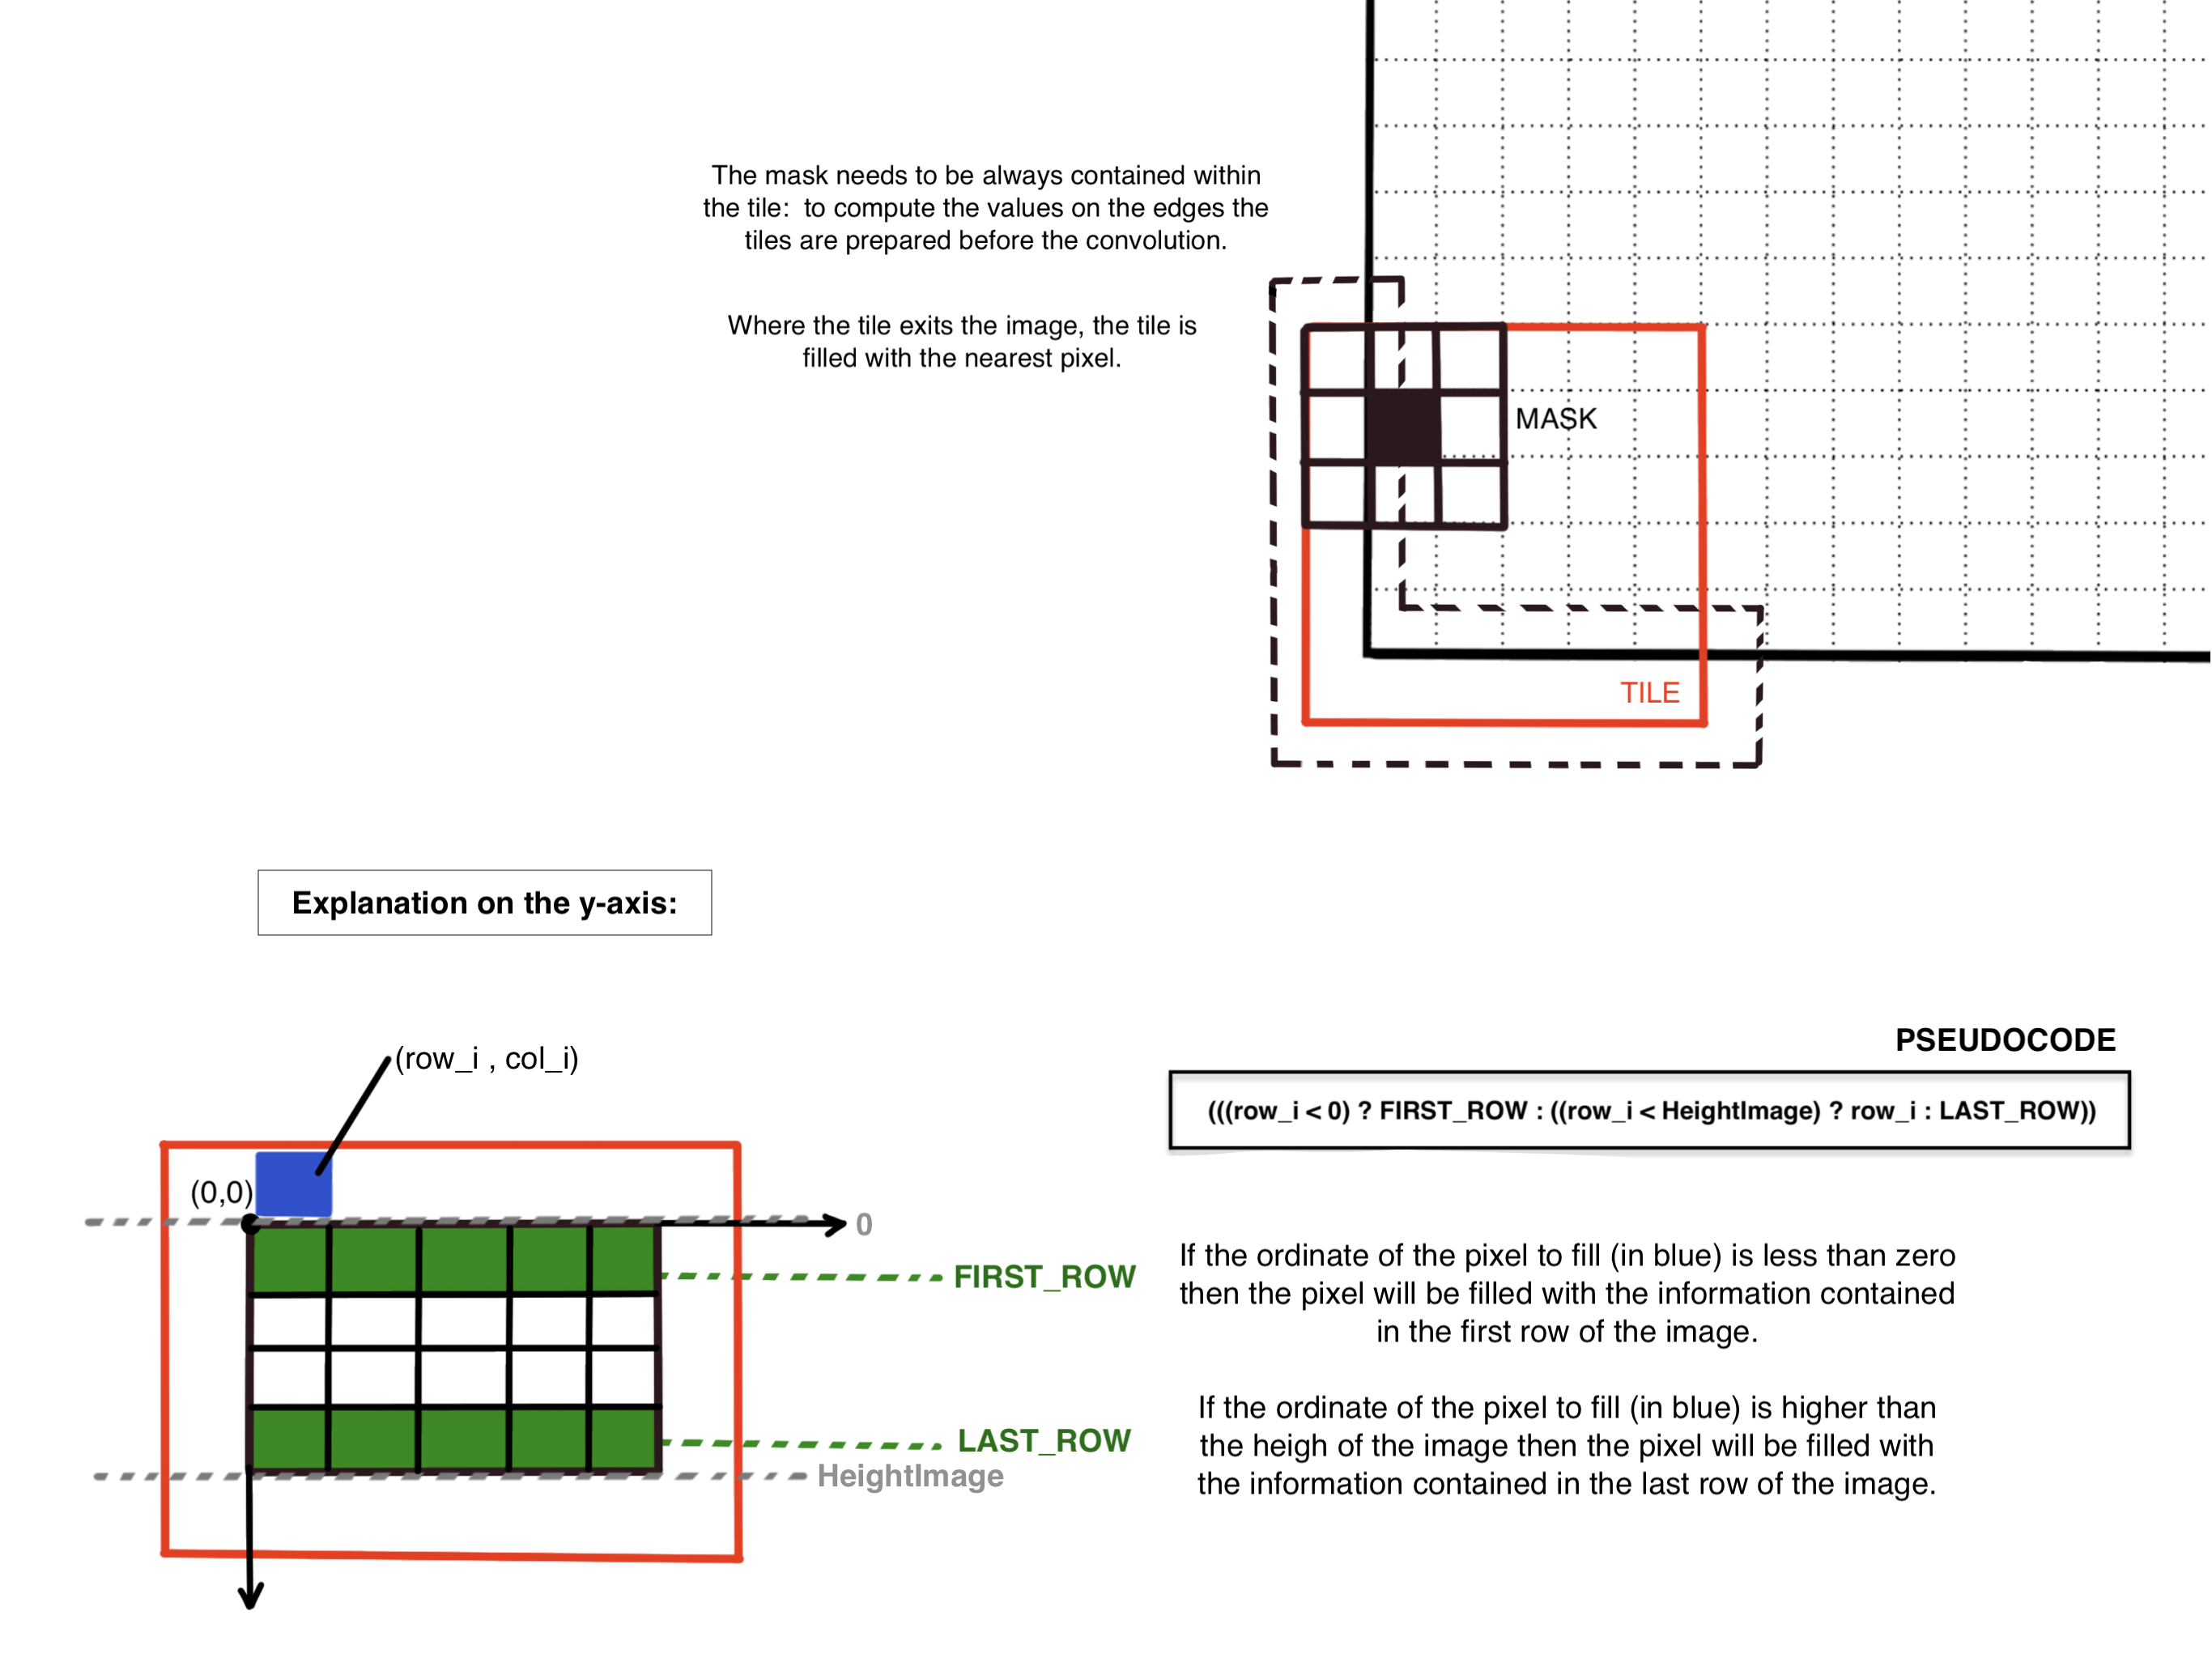
\includegraphics[width=0.75\textwidth]{img/EDGEscheme.png}
        \caption{Border pixel replication (same happens for columns)}
        \label{fig:borderrepl}
    \end{figure}


    \subsection{Image Enhancement}

    This step executes the convolution of the image with the kernel, in order to enhance the image and make it clearer.\\
    Many versions of the algorithm have been tested, starting with a function performing the enhancement using only global memory,
    and then moving to a function using shared memory and a tiling technique.\\
    The first version of the algorithm, which uses only global memory, performs the operations slower than the other,
    but it is the most straightforward one, and it is the one that has been used for the first tests. The possibility to use it if the user
    wants to, is still available. The second version of the algorithm, which uses shared memory, improves the performances of the algorithm, given that the shared memory
    allows to have a faster access to the data. This happens because it is a cache located on chip, and given that it's accessible by all threads of a block,
    it provides a mechanism for threads to cooperate, while diminishing the access to global memory, which is in the DRAM.
    Two main problems arise when using shared memory: the fact that it is limited in size, and it is not possible to use it for all the data that is needed, 
    and bank conflicts, which are caused by the fact that the shared memory is divided into banks, which can be accesses simultaneously by different threads,
    but only if they are accessing different banks. This means that if two threads are accessing the same bank, they will have to wait for the other one to finish,
    and this will cause a slowdown in the execution of the algorithm.
    This is why a tiling technique is used, given that it allows to use the shared memory to its full potential, avoiding conflicts, by using a tiling technique.
    Tiling is a technique that allows to divide the image in tiles, and to perform the convolution on each of them, then combining the results
    of the convolutions in order to obtain the final image. This technique allows avoiding bank conflicts, because each tile is stored in a different
    bank, reducing memory traffic.
    
    The basic version of the algorithm, using a kernel on CPU according to the \textit{Gaussian\_Kernel\_Cpu} function and stored in the \textit{d\_kernel} variable
    allocated in the constant memory, computes the convolution using one thread for each pixel of the image, dividing the image in blocks all of the same size, excluding the last, 
    which can be smaller. The convolution is performed both per color channel and per single block of pixels of the same dimension of the kernel, centered in the pixel to be processed.
    The convolution is performed by multiplying the value of the pixel with the value of the corresponding element of the kernel, and then summing all the results:
    \noindent\begin{lstlisting}[language=C]
...
offsetRow = (idx / dimImgIn + i) * dimImgIn;
offsetCol = idx % dimImgIn + j;
sum += input[offsetRow + offsetCol + 3] * d_kernel[i * dimKernel + j];
...
output[idx] = sum;
...
    \end{lstlisting}

    The second version, with shared memory and tiling, decides if the image is large enough to be tiled by computing the width of the tile:
    \begin{equation}
        widthTile = \sqrt{maxThreadsPerBlock} - (maskDim - 1)
    \end{equation}
    
    \noindent If this value is greater than 1, the tiling technique is used, otherwise the global memory version is used, because the tiling technique would not be efficient
    due to the overhead of the tiling process.
    The shared memory has to be filled first with the color information of the image, then used to perform the convolution with the mask.
    All the initialized threads of the block participate in filling the memory but afterwards only some of them participate in calculating the convolution with the mask for that block.
    The number of threads set for each block corresponds to the number of bytes allocated for the shared memory: in the project it is set to $bigTileDim*bigTileDim$.

    \begin{figure}
        \centering
        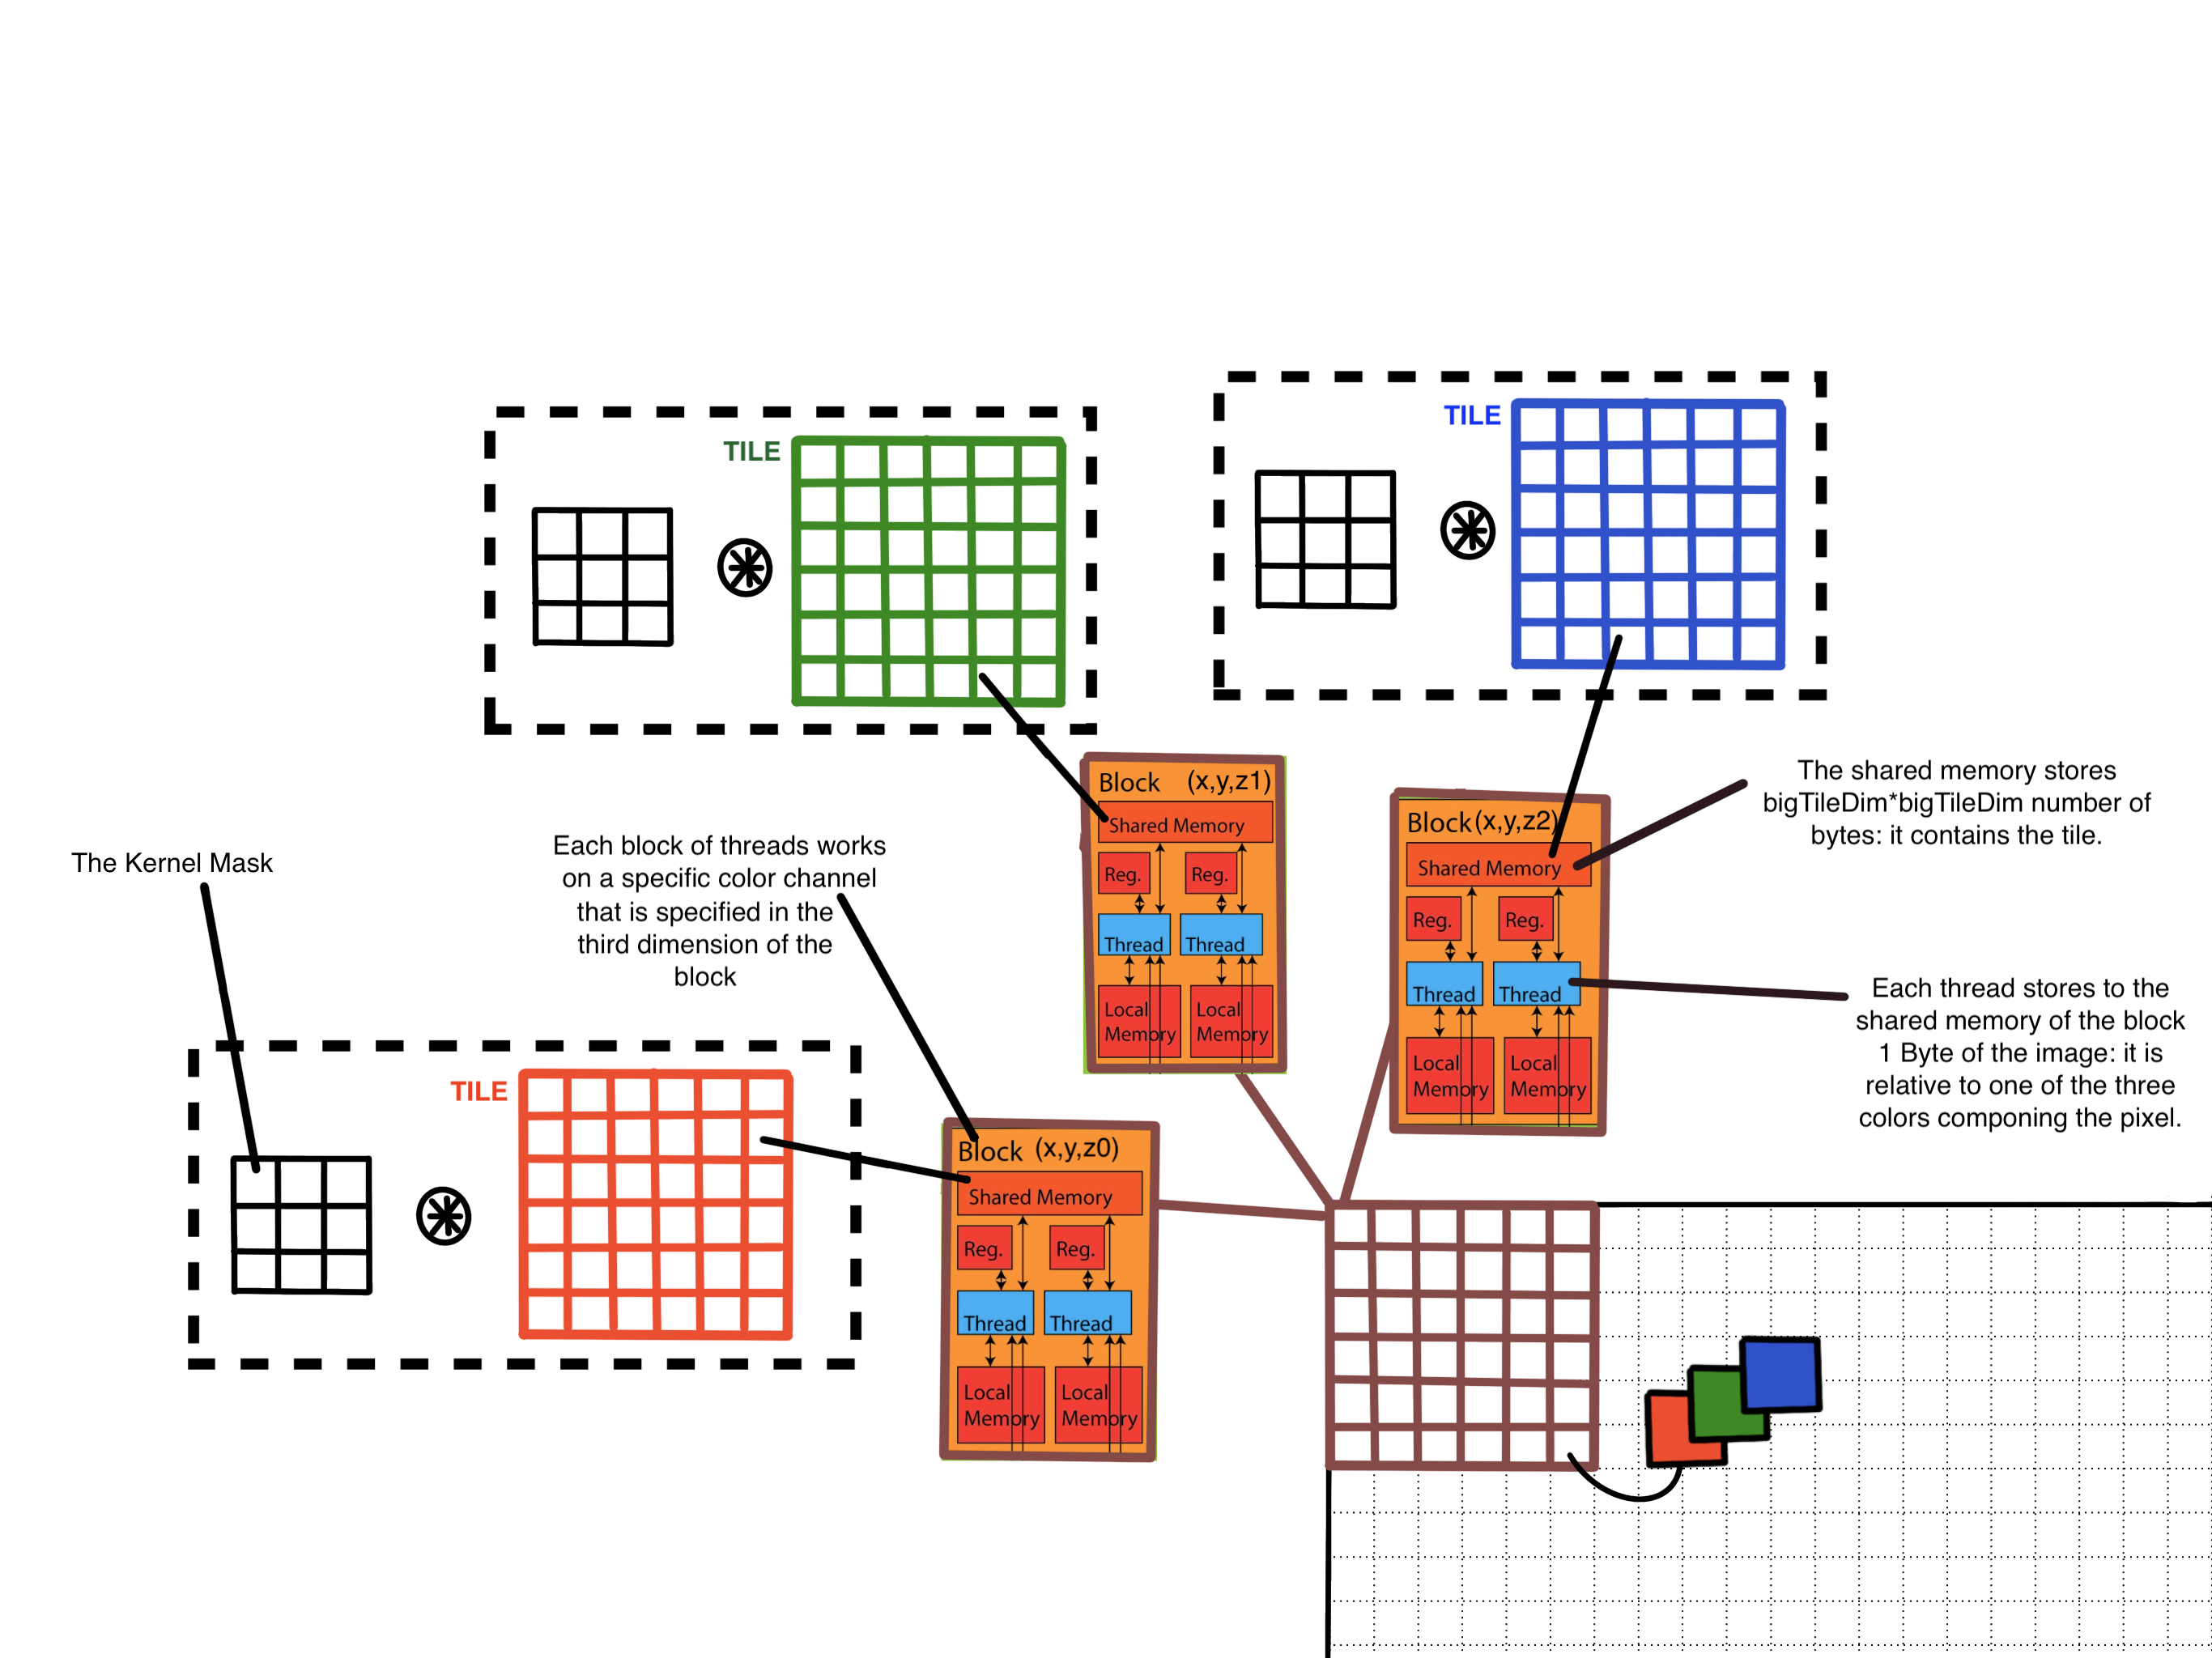
\includegraphics[width=1\textwidth]{img/scheme.png}
        \caption{Schematic representation of enhancement process}
        \label{fig:tiling}
    \end{figure}

    \subsection{Code implementation}
    Taken into consideration what has been said before, the actual implementation has a more direct way of performing the cut, enlargement and convolution.
    The initial version of the algorithm did the cut, the enlargement and the convolution in three different CUDA functions, but this was not the most efficient way of doing it.\\
    The final version, instead, performs the whole process in a single CUDA function, which is called by the main function, and it is the one that is actually executed.
    This function is called \textit{globalCudaUpscaling} in case the global memory version is used, and \textit{tilingCudaUpscaling} in case the shared memory version is possible.

    \begin{figure}[h]
        \centering
        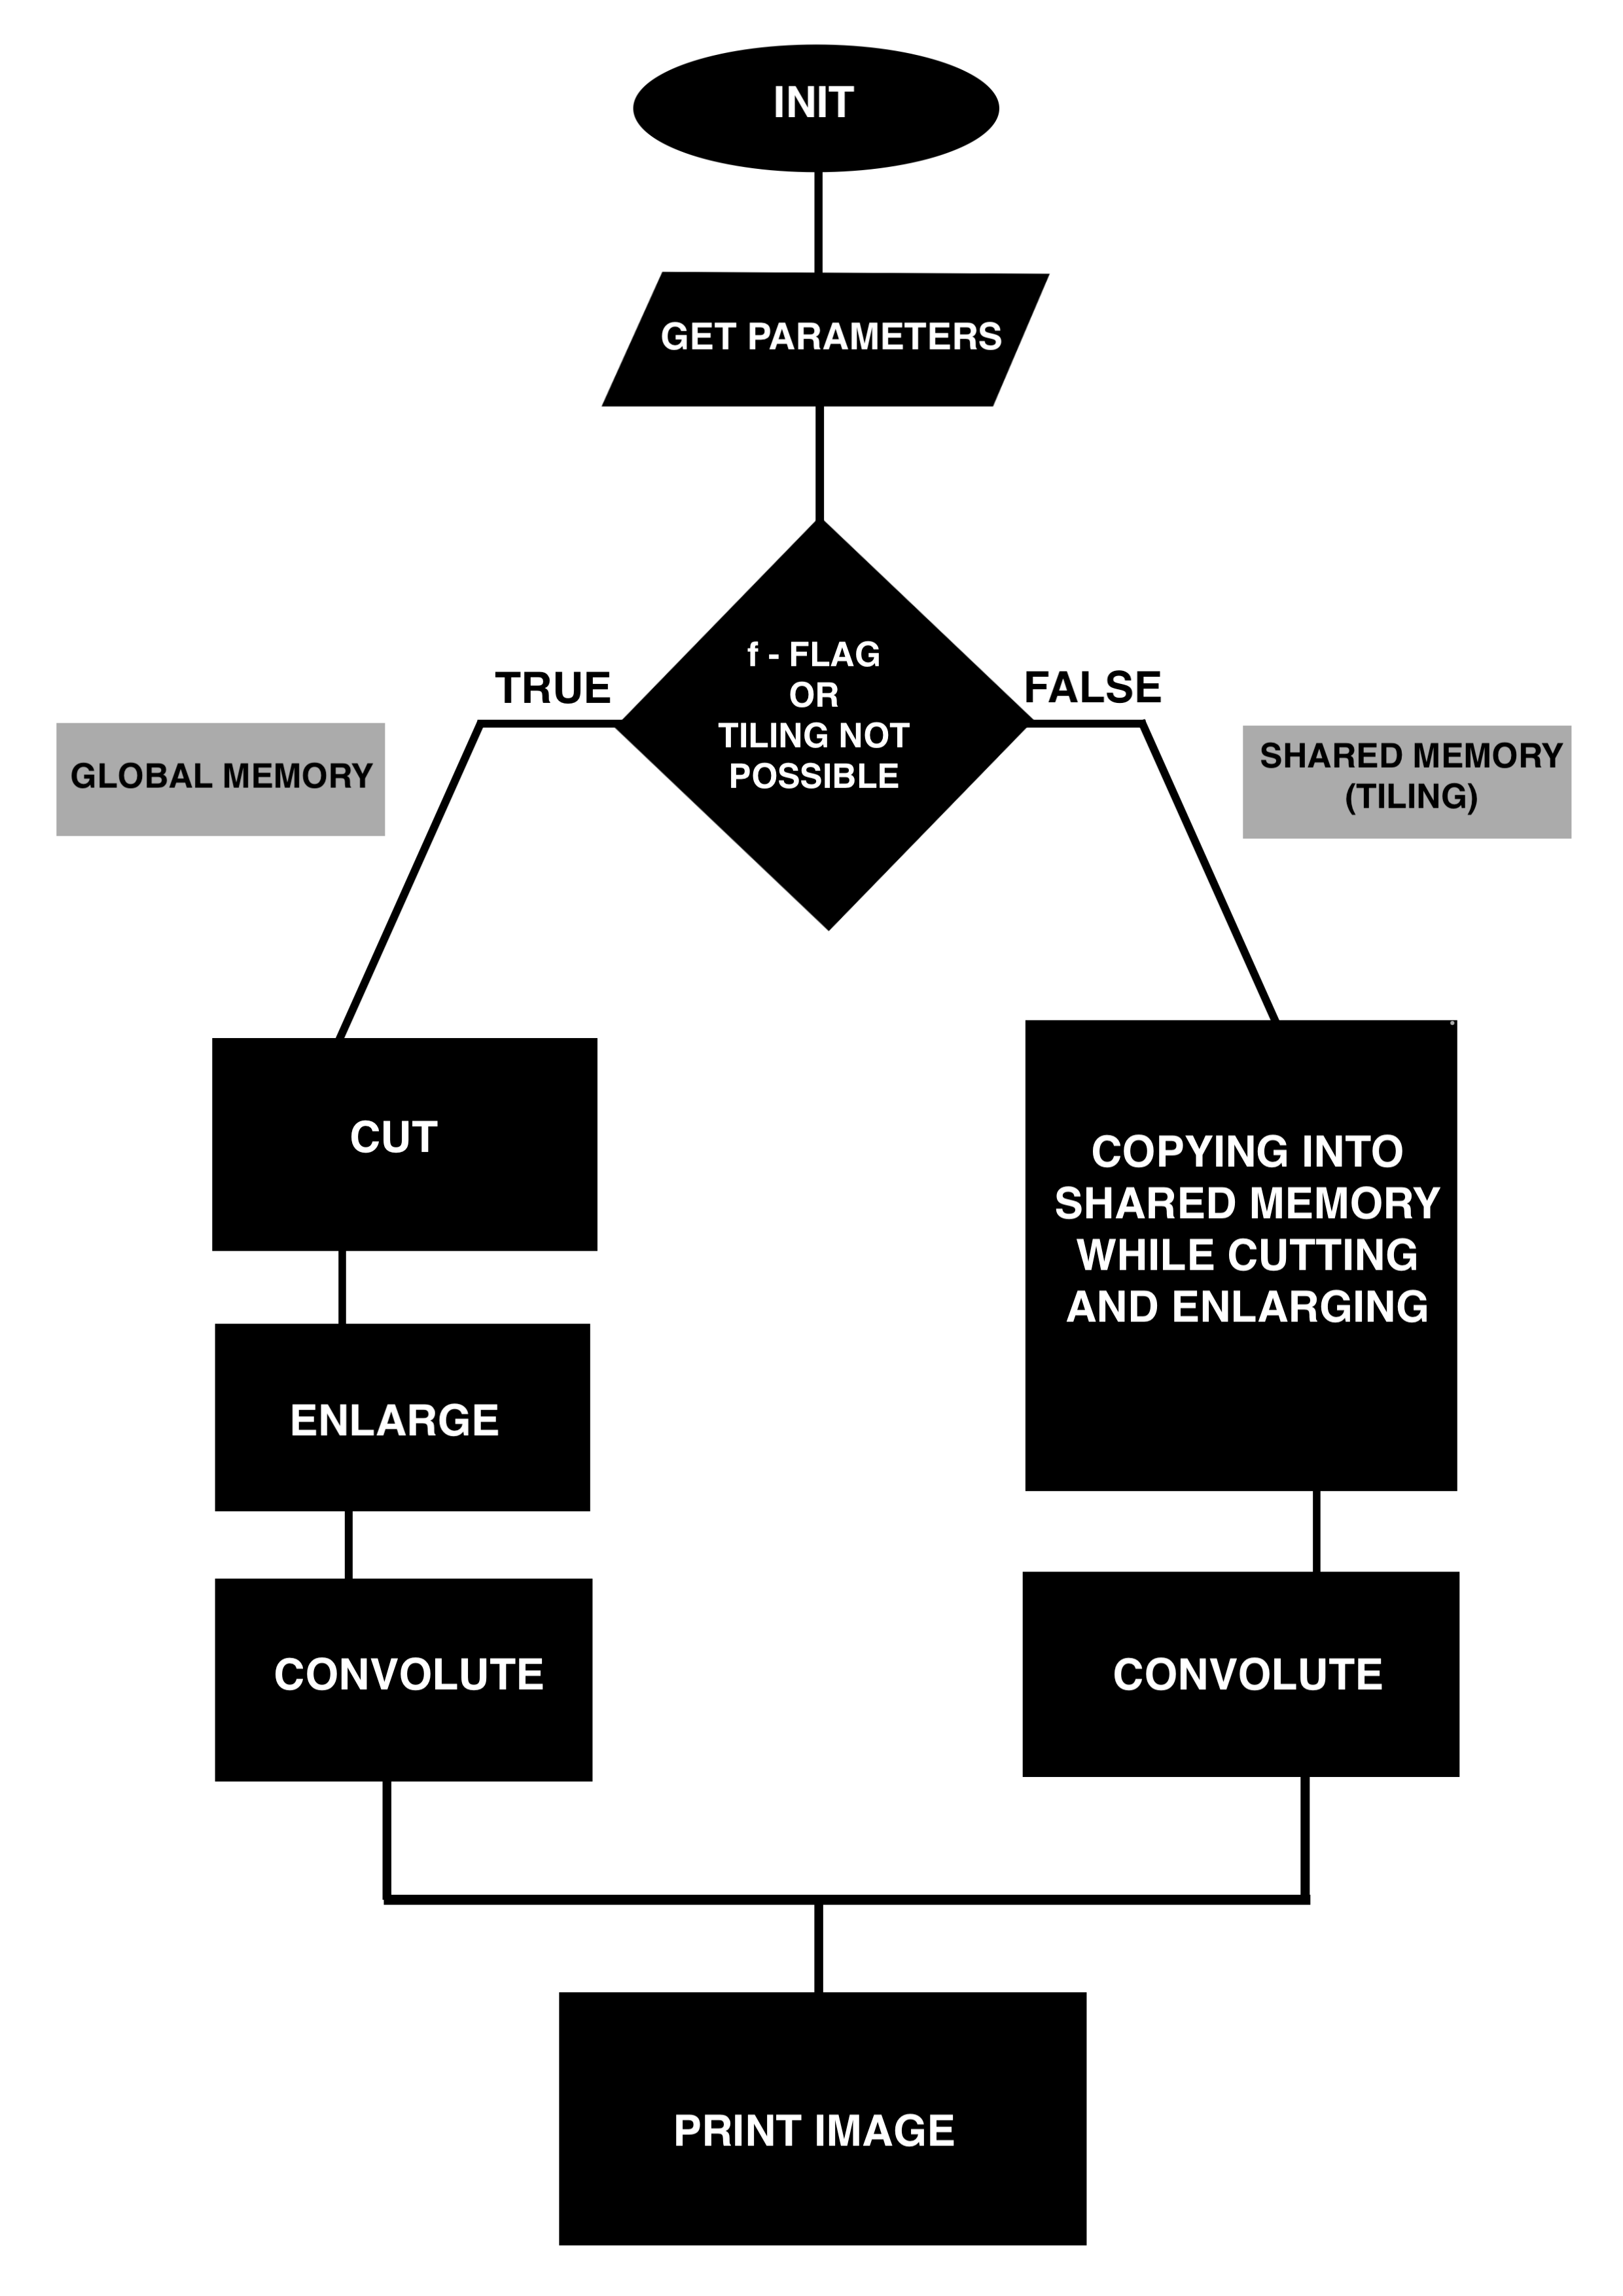
\includegraphics[width=0.7\textwidth]{img/flowchart.png}
        \caption{Flowchart}
        \label{fig:flowchart}
    \end{figure}